\begin{figure*}
% graphic source https://docs.google.com/presentation/d/1CKU1Rtz8Vbk-Std3zFmzBcACf7EBj3amTTOAGKdBluQ
\centering
\begin{minipage}{0.7\linewidth}
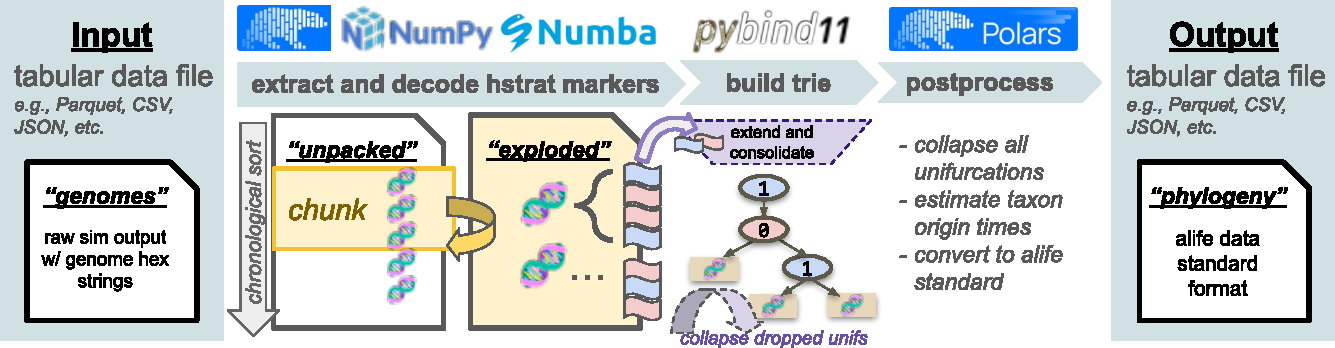
\includegraphics[width=\linewidth]{img/hstratpipeline.pdf}
\end{minipage}
\begin{minipage}{0.1\linewidth}\end{minipage}
\begin{minipage}{0.1\linewidth}\end{minipage}
\begin{minipage}{0.28\linewidth}
\vspace{1em}
\caption{
\textbf{Phylogeny pipeline.}
\small
Hstrat markers are ``unpacked'' from genome hex strings.
Individual markers are decoded into ``exploded'' format.
Inferred trie are progressively extended with genomes, purging dropped unifurcations.
Finally, trie is exported to ALife data standard.
High-performance scientific computing libraries are leveraged to support large datasets.
}
\label{fig:hstratpipeline}
\end{minipage}
\vspace{-1.5em}
\end{figure*}
